\begin{frame}{Króliki Fibonacciego}
    \centering
    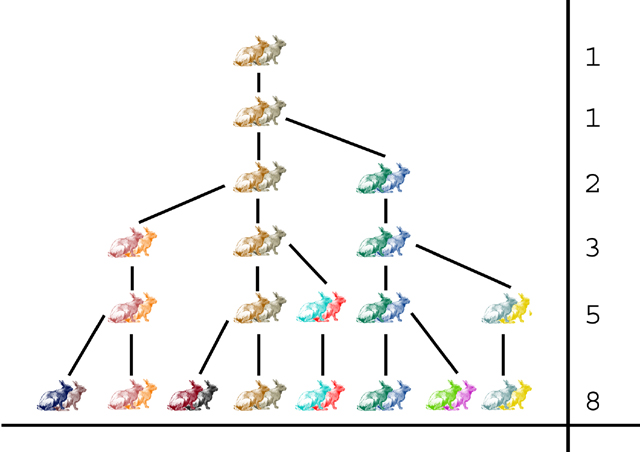
\includegraphics[height=0.8\textheight]{recursion/graphics/fibonacci_rabbits.jpg}
\end{frame}
\begin{frame}[fragile]{Kod w Pythonie}
    \lstinputlisting{recursion/code/fibonacci.py}
\end{frame}
%%%%%%%%%%%%%%%%
\begin{frame}{Stos i drzewo wywołań funkcji}
    \centering
    \begin{columns}
        \begin{column}{0.25\textwidth}
            \textcolor{black}{starting with 5}\\
            \textcolor{black}{starting with 4}\\
            \textcolor{black}{starting with 3}\\
            \textcolor{black}{starting with 2}\\
            \textcolor{black}{starting with 1}\\
            \textcolor{black}{ending with 1}\\
            \textcolor{black}{starting with 0}\\
            \textcolor{black}{ending with 0}\\
            \textcolor{black}{ending with 2}\\
            \textcolor{black}{starting with 1}\\
            \textcolor{black}{ending with 1}\\
            \textcolor{black}{ending with 3}\\
            \textcolor{black}{starting with 2}\\
            \textcolor{black}{starting with 1}\\
            \textcolor{black}{ending with 1}\\
        \end{column}
        \begin{column}{0.25\textwidth}
            \textcolor{black}{starting with 0}\\
            \textcolor{black}{ending with 0}\\
            \textcolor{black}{ending with 2}\\
            \textcolor{black}{ending with 4}\\
            \textcolor{black}{starting with 3}\\
            \textcolor{black}{starting with 2}\\
            \textcolor{black}{starting with 1}\\
            \textcolor{black}{ending with 1}\\
            \textcolor{black}{starting with 0}\\
            \textcolor{black}{ending with 0}\\
            \textcolor{black}{ending with 2}\\
            \textcolor{black}{starting with 1}\\
            \textcolor{black}{ending with 1}\\
            \textcolor{black}{ending with 3}\\
            \textcolor{black}{ending with 5}\\
        \end{column}
        \begin{column}{0.5\textwidth}
            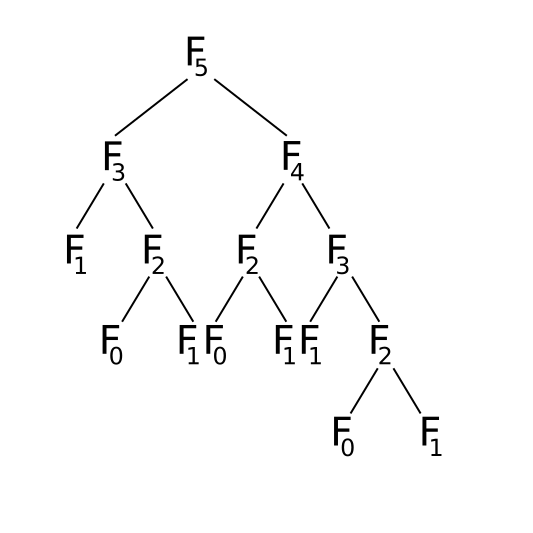
\includegraphics[width=\textwidth]{recursion/graphics/fibonacci_black.png}
        \end{column}
    \end{columns}
\end{frame}
%%%%%%%%%%%%%%%%
\begin{frame}{Stos i drzewo wywołań funkcji}
    \centering
    \begin{columns}
        \begin{column}{0.25\textwidth}
            \textcolor{black}{starting with 5}\\
            \textcolor{black}{starting with 4}\\
            \textcolor{black}{starting with 3}\\
            \textcolor{blue}{starting with 2}\\
            \textcolor{orange}{starting with 1}\\
            \textcolor{orange}{ending with 1}\\
            \textcolor{red}{starting with 0}\\
            \textcolor{red}{ending with 0}\\
            \textcolor{blue}{ending with 2}\\
            \textcolor{black}{starting with 1}\\
            \textcolor{black}{ending with 1}\\
            \textcolor{black}{ending with 3}\\
            \textcolor{blue}{starting with 2}\\
            \textcolor{orange}{starting with 1}\\
            \textcolor{orange}{ending with 1}\\
        \end{column}
        \begin{column}{0.25\textwidth}
            \textcolor{red}{starting with 0}\\
            \textcolor{red}{ending with 0}\\
            \textcolor{blue}{ending with 2}\\
            \textcolor{black}{ending with 4}\\
            \textcolor{black}{starting with 3}\\
            \textcolor{blue}{starting with 2}\\
            \textcolor{orange}{starting with 1}\\
            \textcolor{orange}{ending with 1}\\
            \textcolor{red}{starting with 0}\\
            \textcolor{red}{ending with 0}\\
            \textcolor{blue}{ending with 2}\\
            \textcolor{black}{starting with 1}\\
            \textcolor{black}{ending with 1}\\
            \textcolor{black}{ending with 3}\\
            \textcolor{black}{ending with 5}\\
        \end{column}
        \begin{column}{0.5\textwidth}
            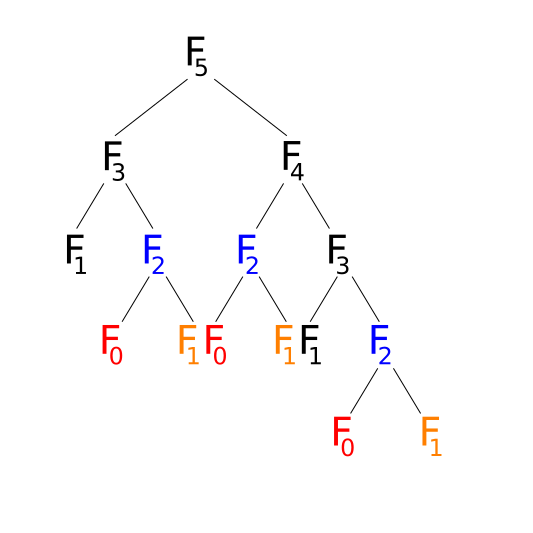
\includegraphics[width=\textwidth]{recursion/graphics/fibonacci_F3.png}
        \end{column}
    \end{columns}
\end{frame}
%%%%%%%%%%%%%%%%
\begin{frame}{Stos i drzewo wywołań funkcji}
    \centering
    \begin{columns}
        \begin{column}{0.25\textwidth}
            \textcolor{black}{starting with 5}\\
            \textcolor{black}{starting with 4}\\
            \textcolor{magenta}{starting with 3}\\
            \textcolor{blue}{starting with 2}\\
            \textcolor{orange}{starting with 1}\\
            \textcolor{orange}{ending with 1}\\
            \textcolor{red}{starting with 0}\\
            \textcolor{red}{ending with 0}\\
            \textcolor{blue}{ending with 2}\\
            \textcolor{green}{starting with 1}\\
            \textcolor{green}{ending with 1}\\
            \textcolor{magenta}{ending with 3}\\
            \textcolor{black}{starting with 2}\\
            \textcolor{black}{starting with 1}\\
            \textcolor{black}{ending with 1}\\
        \end{column}
        \begin{column}{0.25\textwidth}
            \textcolor{black}{starting with 0}\\
            \textcolor{black}{ending with 0}\\
            \textcolor{black}{ending with 2}\\
            \textcolor{black}{ending with 4}\\
            \textcolor{magenta}{starting with 3}\\
            \textcolor{blue}{starting with 2}\\
            \textcolor{orange}{starting with 1}\\
            \textcolor{orange}{ending with 1}\\
            \textcolor{red}{starting with 0}\\
            \textcolor{red}{ending with 0}\\
            \textcolor{blue}{ending with 2}\\
            \textcolor{green}{starting with 1}\\
            \textcolor{green}{ending with 1}\\
            \textcolor{magenta}{ending with 3}\\
            \textcolor{black}{ending with 5}\\
        \end{column}
        \begin{column}{0.5\textwidth}
            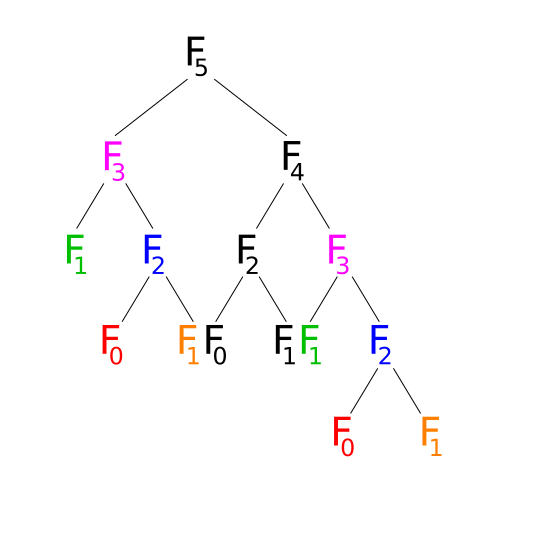
\includegraphics[width=\textwidth]{recursion/graphics/fibonacci_F4.png}
        \end{column}
    \end{columns}
\end{frame}
\begin{frame}{Skierowany graf acykliczny}
    \centering
    \begin{columns}
        \begin{column}{0.5\textwidth}
            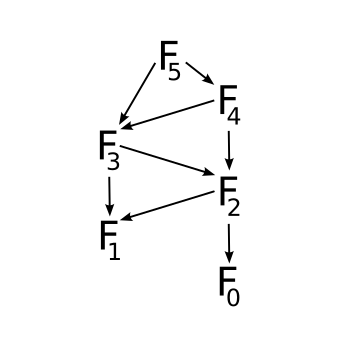
\includegraphics[width=1.2\textwidth,height=0.7\textheight]{recursion/graphics/fibonacci_dag.png}
        \end{column}
        \begin{column}{0.5\textwidth}
            Pewnie zauważyliście, że wiele z funkcji liczy się wielokrotnie dla tych samych danych, co powoduje znaczące wydłużenie działania programu. \\
            Rozwiązaniem tego problemu jest programowanie dynamiczne, prowadzące do drzewa wywołań w formie DAGu, czyli skierowanego grafu acyklicznego.
        \end{column}
    \end{columns}
\end{frame}
%%%%%%%%%%%%%%%%